\chapter{主板相机工程:采集与推流}

\section{主板数据通路总览}

主板把 SC500CS 传感器图像处理为千兆 UDP 码流,ETHB 镜像到显示子板(图~\ref{fig:mainboard})。主链路:SC500CS(MIPI 2lane RAW10,采窗
1287$\times$727,实发 1280$\times$720)$\to$ csi\_unpacket/raw10 解包 $\to$
uial2axis $\to$ line\_retimer(重切 320 拍 $\times$ 720 行)$\to$ group\_fifo
(40.2M $\to$ 100M 跨时钟域)$\to$ cvp\_proc(4:1 位宽变换 + DPC + 去马赛克,
见第 3 章)$\to$ color\_correct(白平衡)$\to$ 七模式风格化 $\to$ pack\_4(攒
96\,bit 组)$\to$ cvp\_eth\_dbg(GMII 125\,M 域字节展开)+ cvp\_gmii\_mac\_tx
$\to$ RGMII $\to$ YT8531 PHY $\to$ ETHA(PC)与 ETHB(镜像,子板)。

\begin{figure}[H]\centering
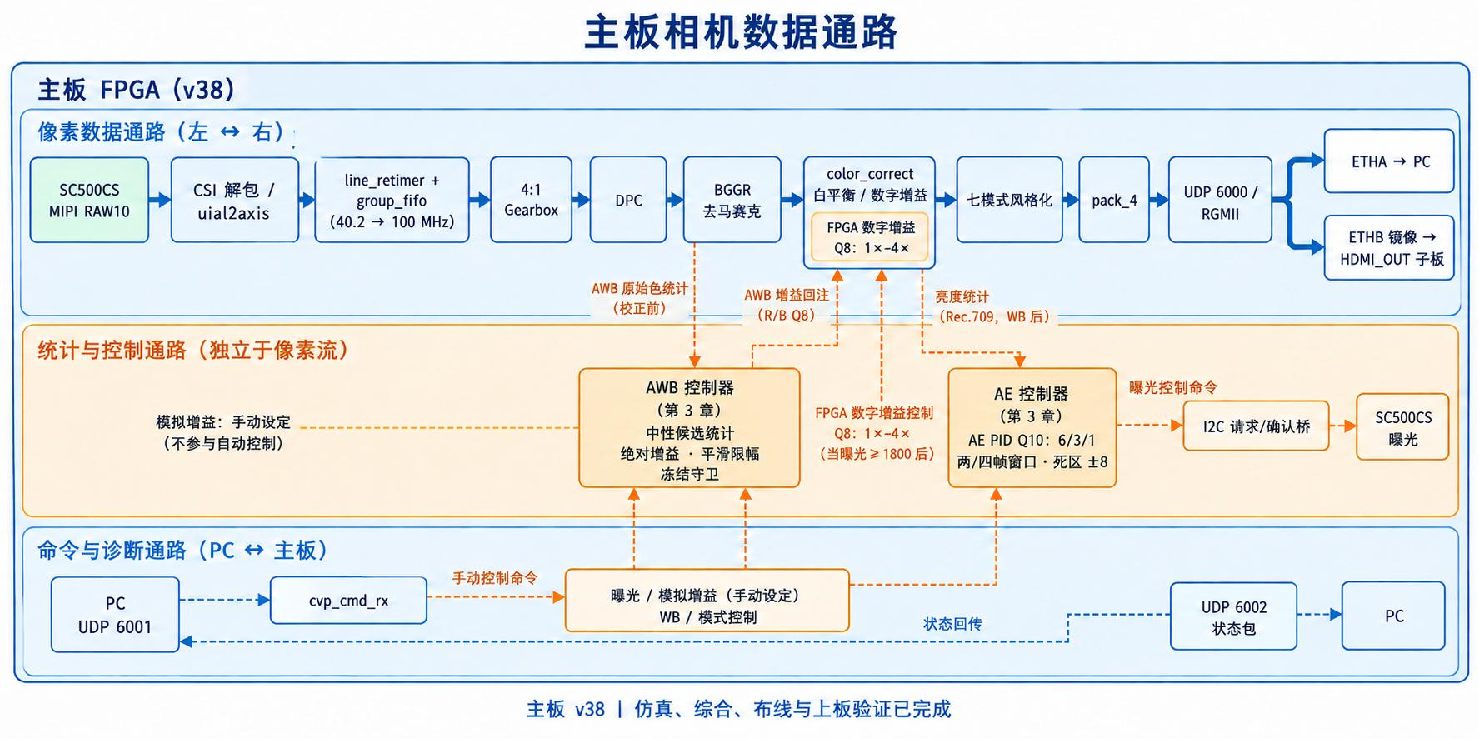
\includegraphics[width=\textwidth]{figs/fig_mainboard.pdf}
\caption{主板数据通路:采集解包 / ISP / 推流 + 命令与状态支路}
\label{fig:mainboard}
\end{figure}

\section{采集与解包层}

采集层负责三件事:传感器配置、MIPI 字节流还原、行帧切分与跨时钟域。传感器工作
参数由 \verb|uics500_cfg/| 配置表(主表/AE 表/SC500GainTbl 增益表,档位 16..143
= 1.0$\times$..15.75$\times$)经 I2C 写入,时序由 uicfgcs500 状态机控制。定版
关键值:VTS=1003 行(30.0\,fps 实测校准);采窗 1287$\times$727 居中于原 1080p
窗,实发 1280$\times$720;默认曝光 500 半行、合法范围 62..1800——曝光上限的原因
是贴近满帧时传感器读出窗相对帧同步偏移数行,720 行窗口的顶部或底部会出现错位带,
1800(900 行)留 103 行裕量;需更亮优先加增益档或补光。

\textbf{行帧切分}:\verb|uial2axis| 整理为 AXI-Stream 并做行/帧切分;
\verb|line_retimer| 把流重切为 320 拍 $\times$ 720 行的规整节拍。这一级有两个
关键实现约束:采窗行数(727)与实发行数(720)是两个不同的参数,不可混淆——用错
会造成帧头漂移、上下半帧互换;行列计数必须与帧起始对齐,否则去马赛克的色平面会
错位。\textbf{跨时钟域}:\verb|group_fifo| 以异步 FIFO 完成 40.2\,MHz 采集域到
100\,MHz 主域的衔接,并统一组格式——下游齿轮箱按"40\,bit(4 像素)/拍"消费,
每拍拿到完整一组。

\textbf{采集健康度}由网口状态上报直接观测(v29 起串口诊断链已移除,由 UDP 6002
状态包替代):状态包含帧计数、组数、流错误与 I2C 诊断,GUI 状态栏实时显示 fps 与
完整率。判定基准:$f=30$、每帧 230{,}400 组;GUI 能收图即采集到推流全链路健康,
收不到图先排查 PC 侧 6000 端口占用(多进程分流是假读数的根源),仍无图再看状态包
帧计数是否走动。摄像头启动带等待与重试机制,并以"第一完整帧"门控后续处理,上电
即出流无需手动干预。

\section{推流层:千兆 UDP 发送}

推流层把 RGB888 像素流打包为千兆 UDP 码流。\verb|pack_4| 攒 4 像素 96\,bit 组;
\verb|cvp_eth_dbg| 在 GMII 125\,MHz 域做字节展开,按\textbf{每帧 1920 包、每包
1440 字节(480 像素)}发送;应用头 6 字节(帧序号、格式字节、4 字节大端偏移 =
包序 $\times$ 1440);以太网帧 1500 字节(ETH14 + IP20 + UDP8 + 头 6 + 数据
1440 + FCS4),目的 MAC 广播、目的 IP 192.168.1.100、端口 6000/6000(状态包
6002)。带宽核算:1920 包 $\times$ 12\,$\mu$s $\approx$ 23.6\,ms/帧 $\to$
30\,fps,线速约 697\,Mbps——必须千兆链路,100M 下必然丢流。

ETHA 与 ETHB 共享同一发送通路,ETHB 输出与 ETHA 完全相同的 RGMII 流(镜像口),
因此 PC 预览、子板回显与状态上报天然一致;两颗 YT8531 各自与对端自协商 1000M。

\section{公共像素流接口(CVP\_PIXEL\_V1)}

风格化与分类挂接点采用统一的 128\,bit 像素字接口:RGB888(23:0)、x/y 坐标
(12 位零起始)、32 位采集帧身份、16 位配置号、8 位模式号、SOF/EOL/EOF 标志
(与对应像素同拍)、错误指示与 OSD/AE/WB 状态位,时钟复位单独传递。摄像头分支
无反压(禁止任意 backpressure),每帧恰 921{,}600 个有效像素、720 个行尾与一个
帧尾。RGB 窗口边界复制、RAW Bayer 窗口反射(保持同色相位)。接口约定保证了点
运算的 RGB 延迟与元数据一致、窗口算子的输出坐标代表实际窗口中心——任何新算法
模块(如分类网络)按此接口即可挂接,不动主链路。

\section{主板显示支路裁剪与状态上报}

v30 起主板移除本地 DDR 帧缓存、显示裁剪与 DSI 发送链,并关闭 7 寸屏背光;
相机、ISP、AE/AWB、UDP 发送、命令接收和状态上报保持工作。ETHB 与 ETHA
仍是同一路 RGMII 发送流的镜像,子板 HDMI 回显因此不依赖主板本地显示硬件。
状态经 UDP 6002 回传,帧计数、RAW 组数、输出长度、I2C 与流错误可供 GUI 诊断。

\section{资源优化与版本状态}

v29 的五项资源优化与差分验证记录如下,作为历史基线;之后 v30 裁剪本地 DDR/DSI
支路,v31--v38 继续更新算法、流恢复与 AE 控制器。当前主板源码为 v38,并非 v29
资源快照。PH1P35MDG324、TD 6.2.168116、100\,MHz 图像时钟的 v38 布线结果为:

\begin{center}\small
\begin{tabular}{lr}
\toprule
指标 & v38 主板版本 \\
\midrule
Slice & 10944 / 21216 (51.58\%) \\
LUT6 / FF & 8807 / 11035 \\
ERAM20K & 51 / 108 \\
DSP & 16 / 40 \\
PLL & 2 / 6 \\
Setup WNS / Hold WNS & +0.119\,ns / +0.020\,ns \\
Setup TNS / Hold TNS & 0 / 0 \\
\bottomrule
\end{tabular}
\end{center}

v38 的 RTL/包校验/Python 回归与 460 帧视频链路模型均通过,当前源码已上板验证。
上表为综合布线报告;AE 控制器仿真对比与板级观测分别记录,本文不把仿真响应当作
板测指标。以下为历史 v29 数据:

主板工程在功能定版(v27)后做了一轮纯资源优化(v29),为应用章的 LeNet 分类网络
腾挪空间,全部改动经新旧实现\textbf{同激励逐位差分}验证,功能与接口不变:

\begin{enumerate}[nosep]
\item \textbf{统计直方图 LUTRAM 化}(cvp\_frame\_stats):32 箱亮度直方图由触发器
阵列改为分布式 RAM,消隐期旋转清扫,走查直读——模块触发器 2312$\to$1044,
F7/F8 多路器清零;
\item \textbf{状态跨域链 ERAM 化}:原 1536\,bit 状态字经三份寄存器跨域传递改为
双 bank ERAM 快照 + 发送期流式读,线上字节序与原实现位精确;
\item \textbf{元数据 FIFO 寄存器化}(风格化/轮廓支路):帧原子元数据的小队列改单
寄存器,腾出 2 块 ERAM20K;
\item \textbf{数据通路摘异步复位}:纯数据延迟链去复位、控制类寄存器保留,统一
触发器控制集;
\item \textbf{移除串口诊断链}:帧率/健康判定改由 UDP 状态包覆盖(见 2.2 节)。
\end{enumerate}

布线结果:Slice 从 17359 降至 15006 (81.8\% 降至 \textbf{70.7\%}),触发器
从 19999 降至 15462 (减少 23\%),LUT 从 14455 降至 12744,ERAM 从 66 降至 65;
Setup WNS +0.102\,ns、Hold WNS +0.020\,ns、TNS 0。回归 22 项全过(v26 套件 12 + v27 套件 6 +
差分 4:统计 17 帧、风格化 14 帧全输出逐位一致,状态链线上包含 CRC 逐字节比对)。
